\section{Introduction and results}

\subsection{Motivation}

%\MS{I would not write a length introduction to complex networks here (because the paper is quite long already and we do not study networks in general in this paper). So, I would remove the first paragraph/list (or incorporate it as a single sentence in the ensuing paragraph). }
%\PvdH{I agree.}

Hyperbolic random graphs were suggested as a suitable model for complex networks by Krioukov et al.~\cite{krioukov2010hyperbolic}, exhibiting the three main characteristics commonly found in complex networks: 
\begin{enumerate}[\upshape 1)]
\item Broad degree distribution (power-law/scale-free),
\item Strong clustering (community structure),
\item Small path lengths (small world phenomenon).
\end{enumerate}
Indeed, in their seminal paper they showed that these graphs have a power-law degree distribution and exhibit strong clustering, while Bringmann et al.~\cite{bringmann2016average} showed that hyperbolic random graphs have doubly logarithmic shortest path lengths. Many other results regarding hyperbolic random graphs have since been established: for instance the existence of efficient routing algorithms~\cite{bringmann2017greedy}, the size of the largest component~\cite{bode2015largest},~\cite{fountoulakis2018law}, [More?] and the number of cliques and the largest clique~\cite{blasius2018cliques}.

The aim of this paper is to study local clustering in hyperbolic random graphs. The first rigorous mathematical analysis of the local clustering coefficient was done by Gugelmann et al.~\cite{gugelmann2012random}. They show~\cite[Theorem 2.1]{gugelmann2012random} that the local clustering coefficient\footnote{Note that in~\cite{gugelmann2012random} this is called the global clustering coefficient. However, since this term is more often associated in the literature with the density of triangles compared to the number of paths of length 2, we use the term local clustering coefficient as is done, for instance, in~\cite{candellero2016clustering}.} is concentrated around its expectation which is shown to be $\bigT{1}$ as the number of vertices tends to infinity. In particular this results implies that the local clustering coefficient is asymptotically bounded away from zero. The convergence of this coefficient was not proven. In contrast, the global clustering coefficient was shown~\cite{candellero2016clustering} to converge in probability to some constant which can be explicitly stated as an integral expression, see Theorem 1.2 in \cite{candellero2016clustering}. The authors mention, however, that their analysis needs significant modification to be able to deal with convergence of the local clustering coefficient.



In addition to the clustering coefficients, an important clustering measure that is often studied is the local clustering function $c(k)$. This function computes for any value of $k$ the average of the local clustering coefficient over all vertices of degree $k$. A general expression of this function for hyperbolic random graphs is given in \cite[Equation (59)]{krioukov2010hyperbolic}. The authors conjecture that as $k$ tends to infinity, $c(k)$ decays as $k^{-1}$, which they observe (Figure 8 in \cite{krioukov2010hyperbolic}) in experiments on the infrastructure of the Internet obtained in~\cite{claffy2009internet}. However, despite the importance of the local clustering function and these interesting observations, its behavior in hyperbolic random graphs had not been completely determined and the following crucial questions regarding clustering in hyperbolic random graphs remained open so far:
\begin{enumerate}[\upshape 1)]
\item Does the local clustering coefficient converge, and if so, what is the limit?
\item What is the limit of the local clustering function and how does it scale with the degree?
\end{enumerate}

In this work we resolve these important open questions. We obtain the asymptotic scaling of $c(k)$ as $k \to \infty$, including the leading constant, as well as an exact expression, in terms of known special functions, of the point-wise limit of the local clustering function as the number of vertices tends to infinity. Interestingly, the scaling of $c(k)$ depends on the exponent of the degree distribution and is only $k^{-1}$ when this exponent exceeds $5/2$. For values less than $5/2$ the scaling is $k^{-s}$ where the value of $s$ depends on the degree distribution exponent. Finally, our analysis allows us to also prove a convergence result for the local clustering coefficient where the limit can again be explicitly expressed in terms of known special functions. 

\PvdH{I recall that J{\'u}lia told me that the results from~\cite{komjathy2018explosion} imply that the local clustering coefficient converges, although they do not mention it in the paper. Should we added a comment related to this?}

\MS{Yes, I think this would probably be good. Either after the sentence `the convergence of this coefficient was not proven' add something like, as you say, the results form .. imply convergence, although not specifically mentioned there. Or drop that sentence about that the convergence was not shown and also rephrase the sentence in 1, to just what is the limit. It should just be clear to the reader that we are not claiming the credit for the convergence itself, but mostly for finding the exact limit (in an analytic expression) and with a very strong sense of convergence. So, let's better emphasize those last two points and hope that they are good enough.}

\subsection{Outline of the paper}

In the next two subsections \ref{ssec:hyperbolic_model} and \ref{ssec:local_clustering} of the introduction, we give the definitions of the hyperbolic random graph and of the local clustering coefficient and function as used in this paper. After this we present our main results in Section \ref{ssec:main_results} and discuss several insights that can be obtained from them and in Section \ref{ssec:simulations} show simulations which confirm these results. Section \ref{sec:proof_outline} contains a detailed high level outline of the proofs of our main results, split up into different propositions. The proofs of these propositions can be found in the last four sections. Section~\ref{sec:concentration_argument} contains a crucial technical result that will be used in the other sections. 

\subsection{Hyperbolic random graphs}\label{ssec:hyperbolic_model}

%, which without loss of generality we take to be $-1$~[CITE]
%The \emph{Poincar\'{e} disc model} for the hyperbolic plane is defined by equipping the open unit disc in $\R^2$ with the metric given by the differential form $\dd s^2 = 4 \frac{\dd x^2 + \dd y^2}{(1 - x^2 - y^2)^2}$.
The hyperbolic plane is an infinite $2$-dimensional manifold with constant negative curvature. Many different representations of the hyperbolic plane exist and we refer to~\cite{anderson2006hyperbolic} \cite{katok1992fuchsian} \cite{beardon2012geometry} for an introduction to hyperbolic geometry.  We will work with the \emph{native representation} of the hyperbolic plane which takes the elements of $\R^2$ in polar coordinates $(r,\theta)$ as the underlying set of points and where distances are determined by the hyperbolic law of cosines.

Let $\alpha > \frac{1}{2}$, $\nu > 0$ and define $R_n = 2\log(n/\nu)$. Then the hyperbolic random graph $G_{\H,n}(\alpha, \nu)$ is defined as follows:
\begin{enumerate}
\item The vertex set if given by $n$ points $u_1, \dots, u_n$ denoted in polar coordinates $(r_i, \theta_i)$, where the angular coordinate $\theta$ is chosen uniformly from $(-\pi,\pi]$ while the radial coordinate $r$ is sampled independently according to the cumulative distribution function
\begin{equation}\label{eq:def_hyperbolic_point_distribution}
	F_{n,\alpha,\nu}(r) = \begin{cases}
		0 &\mbox{if } r < 0\\
		\frac{\cosh(\alpha r)-1}{\cosh(\alpha R_n) - 1} &\mbox{if } 0 \le r \le R_n\\
		1&\mbox{if } r > R_n
	\end{cases}
\end{equation}
\item Any two vertices $u_i=(r_i,\theta_i)$ and $u_j=(r_j,\theta_j)$ are adjacent if and only if $d_\H(u_i,u_j) \le R_n$, where $d_\H$ denotes the distance in the hyperbolic plane, i.e.
\[
	\cosh(r_i) \cosh(r_j) - \sinh(r_i) \sinh( r_j) \cos(|\theta_i-\theta_j|_{2\pi}) \le \cosh(R_n),
\]
as follows from the hyperbolic law of cosines.% rule[CITE?].
\end{enumerate}

\begin{figure}[!t]
\centering
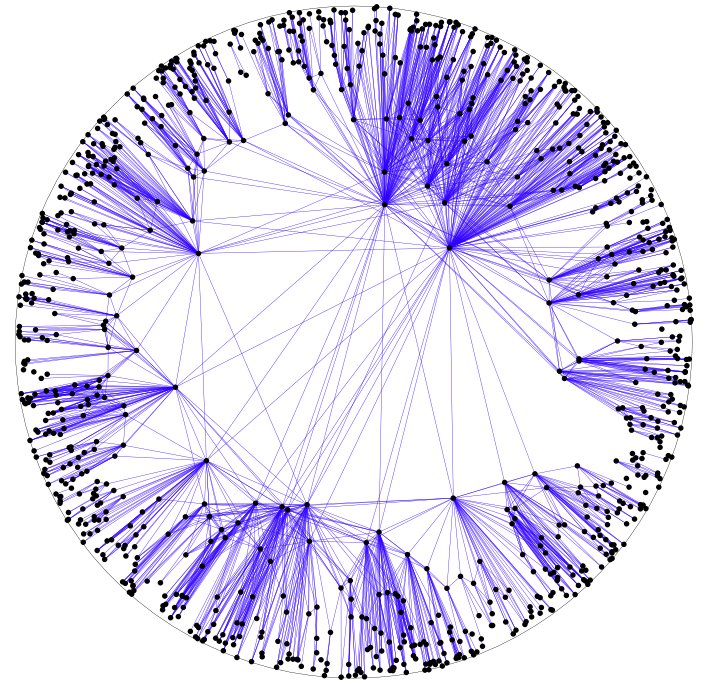
\includegraphics[scale=0.3]{figures/KPKVB.png}
\caption{Example of a Hyperbolic Random Graph $G_{\H,n}(\alpha, \nu)$ with $\alpha = 0.9$, $\nu = 0.2$ and $n = 5000$.
%\PvdH{@Tobias: this figure (HyperRGG\_N5000L5.eps) is taken from the figures you send me. Could you fill in the value of $\alpha$ and $\nu$ you used for the simulation.}
}
\label{fig:H_graph_example}
\end{figure}



Figure~\ref{fig:H_graph_example} shows an example of $G_{\H,n}(\alpha, \nu)$.



%We say that the points $u_i \in G_{\H, n}$ are distributed according to a \emph{$(\alpha, R_n)$-quasi uniform distribution}.



\subsection{Clustering}\label{ssec:local_clustering}

Clustering measures for networks consider the fraction of triangles (triples of connected vertices) in the network. 
For instance, for a simple graph $G$, with vertex set $V(G)$ and edge set $E(G)$, denote by $T_G$ and $\Lambda_G$, respectively, the total number of triangles and the total number of paths of length two in $G$. Then its \emph{global clustering coefficient} is defined as
\[
	c_G = \frac{3 \T_G}{\Lambda_G}.
\]
%This coefficient measures the fraction of triangles in the network compared to the total possible number of triangles. 
A different concept for clustering is defined for each vertex and by taking averages also for the entire graph as well as for all vertices with a specified degree: the \emph{local clustering coefficient} of a vertex $v \in V(G)$ is a real number between zero and one for the extent to which the neighborhood of $v$ resembles a clique. If the vertex $v$ has $k\geq 2$ neighbors, there are ${k \choose 2}$ possible edges between them and its local clustering coefficient is the quotient of the number of these pairs that constitute an existing edge in the graph divided by ${k \choose 2}$. If the vertex $v$ has no or only one neighbor, its clustering coefficient is set to zero. The (average) local clustering coefficient of the graph is the average over the clustering coefficients of all vertices. The local clustering function maps a natural number $k$ to the average over the clustering coefficients of all vertices with degree $k$ if there are vertices with degree $k$ and zero otherwise.

To introduce the notations for these definitions, let $D_G(v)$ denote the degree of vertex $v$ and $N_G(k)$ the number of vertices with degree $k$ in the graph $G$. In addition let $$\T_G(v,v_1,v_2) = \ind{(v,v_1) \in E} \ind{(v, v_2) \in E} \ind{(v_1, v_2) \in E}$$ be the indicator that $v, v_1$ and $v_2$ form a triangle and write
\begin{equation}
	\T_G(v) = \sum_{v_1, v_2 \in V(G)} \T_G(v,v_1,v_2),
\end{equation}
to denote the number of triangles in which node $v$ participates. Then the \emph{local clustering coefficient} is given by
\[
	c_G = \frac{1}{|V(G)|} \sum_{v \in V(G)} \frac{T_G(v)}{\binom{D_G(v)}{2}}.
\]

However, since the local clustering coefficient assigns just one value to the whole network, representing its triangular structure, it is unable to characterize local structural properties involving triangles. The local clustering function, on the other hand, measures the fraction of triangles to which vertices of a given degree belong, compared to the maximum number of triangles in which they could participate~\cite{vazquez2002large,serrano2006clustering}. It describes the triangular structure of vertices in the networks based on their degree and gives a more detailed look at the overall structure of the network. The formal definition of the \emph{local clustering function} is 
\begin{equation}\label{eq:def_local_clustering_general}
	c_{G}(k) = \begin{cases}
		\frac{1}{N_G(k)} \sum_{v \in V(G)}  \ind{D_G(v) = k} \frac{\T_G(v)}{\binom{k}{2}} &\mbox{if } N_G(k) \ge 1\\
		0 &\mbox{else.}
	\end{cases}
\end{equation} 

%We note that other versions of the local clustering function have been considered, for instance where nodes with degree larger than $k$ are considered instead of nodes with degree exactly $k$. \PvdH{Motivate our choice for this local clustering function.} 

\begin{remark}[Notational convention]\label{rmk:notation}
In the remainder of this paper we will compare the local clustering function and many other characteristics between several different graph models. To make notation less cluttered we will often use a unique subscript to identify the graph with respect to which the specific property refers instead of the full graph description. For instance, we shall write $c_{\H,n}(k)$ to denote $c_{G_{\H,n}(\alpha, \nu)}(k)$ and similar, $D_{\H, n}(u)$ for $D_{G_{\H,n}(\alpha, \nu)}(u)$. For the infinite model we will use the subscript $\infty$.
\end{remark}


\subsection{Main results}\label{ssec:main_results}

We are now ready to state our main results for the clustering coefficient and local clustering function in the hyperbolic random graph. When the degree $k$ is a growing function of $n$ we are able to exactly compute the asymptotic behavior of $c_{\H,n}(k)$. 

The results are obtained by coupling the hyperbolic random graph to an infinite random graph $G_\Pcal(\alpha,\nu)$, which we define in Section~\ref{ssec:infinite_model}, and show that the limit of the local clustering coefficient and function for the hyperbolic random graph are given by those for the infinite model. To express these expressions we define for any $y \in \R_+$ 
\[
	\rho(y,k) = \Prob{\Po\left(\xi_{\alpha,\nu} e^{y/2}\right) = k},
\]
where $\xi_{\alpha,\nu} = (4\alpha \nu)/(2\alpha - 1)\pi$ and $\Po(\lambda)$ denotes a Poisson random variable with mean $\lambda$. In addition we define the (marginal) probability measures on $\Rcal := \R_+ \times \R$ by  
\[
	\eta_{y}(x^\prime, y^\prime) = \frac{\alpha \nu e^{-\frac{y}{2}}}{\xi_{\alpha,\nu} \pi} \, \ind{|x^\prime|<e^{(y+y^\prime)/2}} \, e^{-\alpha y^\prime}
\]	
and let
\begin{equation}\label{eq:def_delta_p}
	\Delta_{\Pcal}(y) = \iint_{\Rcal^2} T_\Pcal(y, x_1, x_2, y_1, y_2) \eta_{y}(x_1,y_1)\eta_{y}(x_2,y_2) \dd x_1 \dd x_2  \dd y_1  \dd y_2,
\end{equation}
where 
\[
	T_\Pcal(y, x_1, x_2, y_1, y_2) 
	= \ind{|x_1| \, \le \, e^{(y+y_1)/2}}\ind{|x_2| \, \le \, e^{(y+y_2)/2}}\ind{|x_1-x_2| \, \le \, e^{(y_1+y_2)/2}}.
\]

With these expressions we define the limit local clustering coefficient as
\begin{equation}\label{eq:def_average_clustering_infinite_model}
	c_\infty := \alpha \int_0^\infty \Delta_{\Pcal}(y) (1 - \rho(y,0) - \rho(y,1)) e^{-\alpha y} \dd y,
\end{equation}
while the local clustering function limit is defined as
\begin{equation}\label{eq:def_c_infty_k}
	c_\infty(k) = \frac{\int_0^\infty \rho(y,k) \Delta_\Pcal(y) e^{-\alpha y} \dd y}{\int_0^\infty \rho(y,k) e^{-\alpha y} \dd y}.
\end{equation}

Finally to express the local clustering coefficient and function in the infinite limit model we need a couple of special functions. 

\MS{Here, I would just say that $B(a,b)$ denotes the beta function $B^-(x,a,b)$ the lower incomplete beta function etc. and put/refer to the integral representations in the appendix, as already done for the Meijer-G function.}
%\subsubsection{Special functions}
We let $B(a,b)$ denote the beta-function 
%\[
%	B(a,b) = \int_0^1 t^{a-1}(1-t)^{b-1} \, dt
%\]
and $B^-(x,a,b)$ the lower incomplete beta-function
\[
	B^-(x,a,b) = \int_x^1 t^{a-1}(1-t)^{b-1} \, dt.
\]
In addition we write $\Gamma(z)$ for the Gamma function, $\Gamma^+(q,z)$ for the incomplete Gamma function
\[
	\Gamma^+(q,z) = \int_z^\infty t^{q - 1} e^{-t} \dd t
\]
and define $\Gamma^\ast(q,z) := \Gamma^+(1 + q, z) + \Gamma^+(q, z)$. Finally, we write $U(a,b,z)$ for the hypergeometric U-function (also called Tricomi's confluent hypergeometric function), which for $a,b,z\in \mathbb{C}$, $b \not \in \mathbb{Z}_{\leq 0}$, $\mathrm{Re}(a), \mathrm{Re}(z) >0$ has the integral representation 
\[
	U(a,b,z) = \frac{1}{\Gamma(a)} \int_0^\infty e^{-zt} t^{a-1} (1+t)^{b-a-1} dt,
\] 
see~\cite[p.255 Equation (2)]{erdelyi1953higher}, and let $\MeijerGnew{m}{\ell}{p}{q}{{\bf a}}{{\bf b}}{z}$ denote Meijer's G-Function~\cite{meijer1946gfunction}, see Appendix~\ref{sec:Meijer_G_functions} for more details.

\subsubsection{Local clustering coefficient}

\PvdH{@All: I would be nice if we could show with simulations how close $c_{\H,n}$ actually is to $c_\infty$ for reasonably large $n$ in practice.}

Our first result shows that the local clustering coefficient in the Hyperbolic random graph converges in expectation to $c_\infty$.

\begin{theorem}[Limit for local clustering coefficient in $G_{\H,n}(\alpha,\nu)$] \label{thm:clustering_coefficient_hyperbolic}
Let $\alpha > \frac{1}{2}$, $\nu > 0$. Then,
\[
	\lim_{n \to \infty} \Exp{\left|c_{\H,n} - c_\infty\right|} = 0.
\]
\end{theorem}

Next we establishes the full expression for the clustering coefficient $c_\infty$ in terms of the special function defined above.

\begin{theorem}[Exact expression for clustering coefficient limit]\label{thm:exact_expression_c_infty}
Let $\alpha > \frac{1}{2}$, $\nu > 0$. Then, if $\alpha \ne 1$
\begin{align*}
	c_\infty 
	&=\frac{2 + 4 \alpha + 13 \alpha^2 - 34 \alpha^3 - 12\alpha^4 + 24 \alpha^5}
		{16(\alpha-1)^2 \alpha (\alpha+1) (2\alpha+1)} 
		+  \frac{2^{-1 - 4 \alpha}}{(\alpha - 1)^2} \\
	&\hspace{10pt}+ \frac{(\alpha - 1/2) (B(2 \alpha, 2 \alpha + 1) + B^-(1/2; 1 + 2 \alpha, -2 + 2 \alpha))}
		{2 (\alpha - 1) (3 \alpha - 1)} \\
	&\hspace{10pt}+ \frac{\xi_{\alpha,\nu}^{2\alpha} \Gamma^\ast( - 2 \alpha, \xi_{\alpha,\nu})}{4(\alpha-1)}
		+ \frac{\xi_{\alpha,\nu}^{2\alpha + 2}\alpha (\alpha - 1/2)^2 \Gamma^\ast(- 2 \alpha - 2, \xi_{\alpha,\nu})}
		{2(\alpha-1)^2} \\
	&\hspace{10pt}- \frac{\xi_{\alpha,\nu}^{2\alpha + 1}\alpha (2\alpha - 1) \Gamma^\ast( - 2 \alpha - 1,\xi_{\alpha,\nu})}{(\alpha-1)}
		- \frac{\xi_{\alpha,\nu}^{6\alpha-2}2^{-4\alpha}(3\alpha - 1)\Gamma^\ast( - 6 \alpha + 2, \xi_{\alpha,\nu})}{(\alpha-1)^2}\\
	&\hspace{10pt}-\frac{\xi_{\alpha,\nu}^{6\alpha - 2}(\alpha - 1/2) B^-(1/2; 1 + 2 \alpha, -2 + 2 \alpha)\Gamma^\ast( - 6 \alpha + 2, \xi_{\alpha,\nu})}{(\alpha-1)} \\
	&\hspace{10pt}- \frac{e^{-\xi_{\alpha,\nu}} \Gamma(2\alpha+1) 
		\left(U(2\alpha+1,1-2\alpha,\xi_{\alpha,\nu}) + U(2\alpha+1,2-2\alpha,\xi_{\alpha,\nu})\right)}{4(\alpha-1)} \\
	&\hspace{10pt}+ \frac{\xi_{\alpha,\nu}^{6\alpha - 2} \Gamma(2\alpha+1)\left( 	
		\MeijerGnew{3}{0}{2}{3}{1,3-2\alpha}{3-4\alpha,-6\alpha+2,0}{\xi_{\alpha,\nu}}
		+ \MeijerGnew{3}{0}{2}{3}{1,3-2\alpha}{3-4\alpha,-6\alpha+3,0}{\xi_{\alpha,\nu}}\right)}{4(\alpha-1)},
\end{align*}
while for $\alpha = 1$,
\begin{align*}
	c_\infty &= \frac{575 - 12 \pi^2}{576} + \frac{\eta^4(7 + \pi^2)\Gamma^\ast(-4, \eta)}{4}\\
	&\hspace{10pt}- \frac{1}{2} \int_0^1 (1 - 4z + 3z^3)\log(1-z)(z + \eta)e^{-\eta/z} \dd z\\
	&\hspace{10pt}- \int_0^1 \Li_2(z)(z^3 + \eta z^2) e^{-\eta/z} \dd z,		
\end{align*}
with $\eta = 4\nu/\pi$ and $\Li_2(z) = \sum_{t = 1}^\infty z^t/t^2$, the dilogarithm function\footnote{Note that the integrals in the expression for $c_\infty$ for $\alpha = 1$ exists: for the first one note that $1-4z+3z^2=(1-z)(1-3z)$, so the integrand can be bounded by $C(1-z)\log(1-z)$ on $[0,1)$ for some constant $C$, which can be continued continuously to the compact interval $[0,1]$ by noting that the limit for $z \rightarrow 1$ is zero, so the integrand is bounded on a bounded domain and hence, this integral is finite; for the second integral note that $\Li_2(z)$ is bounded by $\Li_2(1)$ on $[0,1]$, which is a series with well-known finite limit, so again the integrand is bounded on a bounded domain and hence the second integral is also finite.}. 
\end{theorem}




\subsubsection{Local clustering function}

We obtain similar results for the local clustering function. The first states that $c_{\H,n}(k)$ is asymptotically equivalent to $c_\infty(k)$ in an $L^1$ sense.

\begin{theorem}[Limit for local clustering function in $G_{\H,n}(\alpha, \nu)$]
\label{thm:asymptotic_local_clustering_hyperbolic}
Let $\alpha > \frac{1}{2}$, $\nu > 0$ and $(k_n)_{n \ge 1}$ be any positive sequence, possibly constant, such that $k_n = \smallO{n^{\frac{1}{2\alpha + 1}}}$. Then, 
\[
	\lim_{n \to \infty} \Exp{\left|\frac{c_{\H,n}(k_n)}{c_\infty(k_n)} - 1\right|} = 0.
\]
%where
%\[
%	C_{\alpha,\nu} = \begin{cases}
%		C_\alpha \left(\frac{2\alpha \nu}{\pi\left(\alpha - \frac{1}{2}\right)}\right)^{4\alpha - 2}
%		&\mbox{if } \frac{1}{2} < \alpha < \frac{3}{4},\\
%		\frac{2\alpha \nu}{\pi\left(\alpha - \frac{1}{4}\right)} &\mbox{if } \alpha = \frac{3}{4},\\
%		\frac{2\alpha \nu}{\pi\left(\alpha - \frac{3}{4}\right)} &\mbox{if } \alpha \ge \frac{3}{4}
%	\end{cases} 
%\]
%with $C_\alpha$ as defined in \eqref{eq:def_C_alpha}.
\end{theorem}

Next we give an exact expression for $c_\infty(k)$ in terms of the special functions defined earlier.

\begin{theorem}[Exact expression for local clustering function limit]
\label{thm:exact_expression_local_clustering}
Let $\alpha > \frac{1}{2}$, $\nu > 0$. Then, for $\alpha \ne 1$
\begin{align*}
	c_\infty(k) 
	&= \frac{\xi_{\alpha,\nu}^{4\alpha - 2}\Gamma^+(k-6\alpha + 2,\xi_{\alpha,\nu})}{\Gamma^+(k-2\alpha,\xi_{\alpha,\nu})}
		\left(\frac{2^{-4\alpha - 1}(3\alpha - 1)}{\alpha(\alpha - 1)^2} + \frac{(\alpha - \frac{1}{2})B^-\left(\frac{1}{2},2\alpha + 1, 2\alpha - 2\right)}{2\alpha(\alpha - 1)}\right)\\
	&\hspace{10pt}- \frac{\xi_{\alpha,\nu}^{4\alpha - 2}\Gamma(2\alpha + 1)}{\Gamma^+(k-2\alpha,\xi_{\alpha,\nu})}
		\MeijerGnew{3}{0}{2}{3}{1,3-2\alpha}{3-4\alpha,-6\alpha+k+2,0}{\xi}\\
	&\hspace{10pt}+ \frac{1}{8\alpha(\alpha - 1)}
		\left(\frac{\xi_{\alpha,\nu}^{k-2\alpha}e^{-\xi}U(2\alpha+1,1+k-2\alpha,\xi_{\alpha,\nu})}
		{\Gamma^+(k-2\alpha,\xi_{\alpha,\nu})}-1\right)\\
	&\hspace{10pt}- \frac{(\alpha - 1/2)^2 \xi_{\alpha,\nu}^2 \Gamma^+(k-2\alpha -2,\xi_{\alpha,\nu})}
		{4(\alpha - 1)^2 \Gamma^+(k-2\alpha,\xi_{\alpha,\nu})}
\end{align*}
while for $\alpha = 1$
\begin{align*}
	c_\infty(k) &= \frac{9 \eta^3}{2 k!} 	
		\Gamma^+(k-3,\eta)-\frac{\xi_{\alpha,\nu}^4}{k!}\frac{7+\pi^2}{4}\Gamma^+(k-4,\eta)\\
	&\hspace{10pt}+ \frac{\eta^k}{2k!}\int_0^1 (1-4z+3z^2)\ln(1-z)z^{1-k}e^{-\eta/z}\dd z\\ 
	&\hspace{10pt}+ \frac{\eta^k}{k!}\int_0^1 z^{3-k} \Li_2(z) e^{-\eta/z} \dd z,
\end{align*}
with $\eta = 4\nu/\pi$ and $\Li_2(z) = \sum_{t = 1}^\infty z^t/t^2$, the dilogarithm function.
\end{theorem}

From the exact expression for $c_\infty(k)$ we obtain its asymptotic behavior as $k \to \infty$. For this we first define, for any $\frac{1}{2} < \alpha < \frac{3}{4}$,
\begin{equation}\label{eq:def_C_alpha}
	C_\alpha = \frac{2^{-4\alpha - 1}(3\alpha - 1)}{\alpha(\alpha-1)^2} 
	+ \frac{\alpha - \frac{1}{2}}{2(\alpha - 1)\alpha} B^-(\frac{1}{2},2\alpha + 1, 2\alpha - 2)
	- \frac{1}{4(\alpha - 1)}B(2\alpha, 3\alpha - 4).
\end{equation}
Moreover, to simplify the statement we define the scaling function 
\begin{equation}\label{eq:def_scaling_function}
s_\alpha(k_n) = \begin{cases} 
		k^{4\alpha-1} &\frac{1}{2}<\alpha<\frac{3}{4}, \\
		\frac{k}{\log(k)} & \alpha = \frac{3}{4}, \\
		k &\alpha > \frac{3}{4}.
\end{cases}
\end{equation}

We now have the following result, where the constant $C_\alpha$ emerges when we consider the local clustering function for $\frac{1}{2} < \alpha < \frac{3}{4}$.

\begin{theorem}[Asymptotic behavior of local clustering function limit]\label{thm:asymptotics_average_clustering_P}
Let $\alpha > \frac{1}{2}$, $\nu > 0$. Then,
\[
	\lim_{k \to \infty} \frac{c_\infty(k)}{s_\alpha(k)} 
	= \begin{cases}
			C_\alpha \left(\frac{4\alpha \nu}{\pi\left(2\alpha - 1\right)}\right)^{4\alpha - 2}
			&\mbox{if } \frac{1}{2} < \alpha < \frac{3}{4},\\
			\frac{3 \nu}{\pi} &\mbox{if } \alpha = \frac{3}{4},\\
			\frac{8\alpha \nu}{\pi\left(4\alpha - 3\right)} &\mbox{if } \alpha \ge \frac{3}{4},
	\end{cases}
\]
with $C_\alpha$ as defined in \eqref{eq:def_C_alpha}.
\end{theorem}

The following is an immediate consequence of Theorem~\ref{thm:asymptotic_local_clustering_hyperbolic} and Theorem~\ref{thm:asymptotics_average_clustering_P}.

\begin{corollary}[Asymptotic behavior of local clustering function in $G_{\H,n}(\alpha,\nu)$]
Let $\alpha > \frac{1}{2}$, $\nu > 0$, $(k_n)_{n \ge 1}$ be any positive sequence such that $k_n \to \infty$ and $k_n = \smallO{n^{\frac{1}{2\alpha + 1}}}$ and $s_\alpha(k)$ defined as in~\eqref{eq:def_scaling_function}. Then, as $n \to \infty$,
\[
	\frac{c_{\H,n}(k_n)}{s_\alpha(k_n)} \, \stackrel{L^1}{\rightarrow} \, 
	\begin{cases}
				C_\alpha \left(\frac{4\alpha \nu}{\pi\left(2\alpha - 1\right)}\right)^{4\alpha - 2}
				&\mbox{if } \frac{1}{2} < \alpha < \frac{3}{4},\\
				\frac{3\nu}{\pi} &\mbox{if } \alpha = \frac{3}{4},\\
				\frac{8\alpha \nu}{\pi\left(4\alpha - 3\right)} &\mbox{if } \alpha \ge \frac{3}{4},
		\end{cases}
\]
where $\stackrel{L^1}{\to}$ denotes converges in expectation.
\end{corollary}

This result completely characterizes the asymptotic behavior of the local clustering function in Hyperbolic Random Graphs. In particular we observe that the conjectured scaling of $k^{-1}$ from~\cite{krioukov2010hyperbolic} only occurs when $\alpha > 3/4$, or equivalently, when the exponent of the pdf of the degree distribution is larger than $5/2$. 

\PvdH{@All: It would be nice if we could add some simulations showing this scaling in practice, especially the different regimes.}

The majority of the paper is dedicated to prove Theorem~\ref{thm:asymptotic_local_clustering_hyperbolic}, which is based on a sequence of subsequent results for the local clustering function in related random graph models and Theorem~\ref{thm:asymptotics_average_clustering_P}. The exact flow of the argument is explained in Section \ref{sec:proof_outline}. The proof for Theorem~\ref{thm:asymptotic_local_clustering_hyperbolic}, using these results, can be found in Section \ref{ssec:proof_main_results}. Here we also give the proof of Theorem~\ref{thm:clustering_coefficient_hyperbolic}. The exact result for the local clustering coefficient and function, as well as the proofs of Theorem~\ref{thm:exact_expression_c_infty} and~\ref{thm:asymptotics_average_clustering_P} can be found in Section~\ref{sec:asymptotics_average_clustering_ast_P}.

We end this section with some important observations regarding local clustering in hyperbolic random graphs.

\PvdH{Populate these paragraphs}

\paragraph{Transition in the scaling of local clustering}
%Note that Theorem \ref{thm:asymptotic_local_clustering_hyperbolic} implies that for $\frac{1}{2} < \alpha < \frac{3}{4}$ the local clustering $c_{\H,n}(k)$ decays as $k^{-(4\alpha - 2)}$ while for $\alpha > \frac{3}{4}$ it is $k^{-1}$.

\paragraph{Maximum scaling for $k_n$ is $n^{\frac{1}{2\alpha +1}}$}
All our results for clustering in the hyperbolic random graph are valid for any sequence $k_n$ such that $k_n = \smallO{n^{\frac{1}{2\alpha + 1}}}$. Although one would like to have results for any sequence $k_n \le n$, it turns out that $n^{1/(2\alpha + 1)}$ is the optimal scaling for which Theorem~\ref{thm:clustering_coefficient_hyperbolic} can be true. To see why this is the case note that by definition of the local clustering function~\eqref{eq:def_local_clustering_general} we have that $c_{\H,n}(k_n) = 0$ if $N_{\H,n}(k_n) = 0$. Hence, it follows by Markov's inequality that for any positive function $f$
\begin{align*}
	\Exp{\left|\frac{c_{\H,n}(k_n)}{f(k_n)} - 1\right|} 
	&\ge \Prob{N_{\H,n}(k_n) = 0} \ge 1 - \Exp{N_{\H,n}(k_n)}.
\end{align*}
We shall later establish (see Lemma [??] \PvdH{Find the reference for this Lemma}) that $\Exp{N_{\H,n}(k_n)} = \bigT{n k_n^{-(2\alpha + 1)}}$. Therefore if $k_n$ is such that $k_n = \omega\left(n^{\frac{1}{2\alpha + 1}}\right)$ we have
\[
	\lim_{n \to \infty} n k_n^{-(2\alpha + 1)} 
	= \lim_{n \to \infty} \left(n^{-\frac{1}{2\alpha + 1}} k_n\right)^{-(2\alpha + 1)} = 0
\]
and hence
\[
	\lim_{n \to \infty} \Exp{\left|\frac{c_{\H,n}(k_n)}{f(k_n)} - 1\right|} 
	\ge \lim_{n \to \infty} 1 - \Exp{N_{\H,n}(k_n)} = \lim_{n \to \infty} 1 - \bigT{n k_n^{-(2\alpha + 1)}} = 1 \ne 0,
\]
for any positive function $f$. This implies that we cannot expect a result like that of Theorem~\ref{thm:clustering_coefficient_hyperbolic} to hold as soon as $k_n = \omega\left(n^{\frac{1}{2\alpha + 1}}\right)$.


%Maybe, it would make sense to incorporate this statement into theorem \ref{thm:asymptotic_local_clustering_hyperbolic}, i.e. that the asymptotic behaviour of $c(k_n)$ is not well-defined for $k_n \gg n^{\frac{1}{2\alpha+1}}$? Resp. claim that a.a.s. the number of vertices of degree $k_n \gg n^{\frac{1}{2\alpha+1}}$ is zero, such that taking the average over these is not well-defined.

\paragraph{Universality of scaling transition}

\paragraph{Geometric inhomogeneous random graphs}

%\paragraph{Local clustering for growing versus fixed degrees}
%%The main difference between Theorem \ref{thm:fixed_local_clustering_hyperbolic} and Theorem \ref{thm:asymptotic_local_clustering_hyperbolic} is that for fixed degrees $k$ we have a small correction term that depends on the value $k$. 
%
%\MS{We note that the above statements / theorems are disjoint: in one case the degree is fixed corresponding to a constant sequence and in this case the error only depends on $n$, whereas in the other case, the degrees are assumed to be increasing, so in particular unbounded resp. tending to infinity and only the leading term in the asymptotic expansion w.r.t. $k_n \rightarrow \infty$ is given. This allows to study vertices of relatively high degree, e.g. close to the maximum degree (note that there are a.a.s. no vertices with degree exactly the expected maximum degree of $k_n = n^{\frac{1}{2\alpha}}$).}

%The main difference between Theorem \ref{thm:fixed_local_clustering_hyperbolic} and Theorem \ref{thm:asymptotic_local_clustering_hyperbolic} is that for fixed degrees $k$ we have a small correction term that depends on the value $k$. 

\subsection{Simulations}\label{ssec:simulations}